%!TeX program = xelatex

\documentclass[fontsize=13.0pt, oneside, a4paper, openany, vietnamese, english]{Thesis}
% Set sans serif font to Arial
%\setsansfont{Arial}
% Set serifed font to Times New Roman
%\setmainfont{Times New Roman}
\title{Tên đề tài}
\usepackage[backend=bibtex,bibstyle=thesis,sorting=nyvt,block=none,defernumbers=true,autolang=other]{biblatex}

% Package generate lorem text
\usepackage{lipsum}

\addbibresource{Refs.bib}

\begin{document}
    % Trang bìa
    % Nếu là tiếng Việt
    \begin{titlepage}
	\begin{tikzpicture}[remember picture, overlay]
	\draw[line width = 2pt] ($(current page.north west) + (1.3in,-1.1in)$) rectangle ($(current page.south east) + (-0.7in,1.1in)$);
	\end{tikzpicture}
	%\vspace*{-1.15cm}
	\vspace*{-0.7cm}
	\begin{center}
		% Upper part of the page
		{\bfseries ĐẠI HỌC QUỐC GIA TP.HCM}\\
		{\bfseries TRƯỜNG ĐẠI HỌC KHOA HỌC TỰ NHIÊN }\\
            {\bfseries KHOA TOÁN - TIN HỌC }\\[3.0cm]


		{\large \bfseries LÊ NHỰT NAM \hspace{1.00em}}\\[2.7cm]


		{ \bfseries \large XẤP XỈ ĐẠO HÀM \\BẰNG ĐẠO HÀM CỦA ĐA THỨC NỘI SUY}\\[2.4cm]
		{\bfseries TIỂU LUẬN GIẢI TÍCH SỐ}\\[6.5cm]

		%\vfill

		% Bottom of the page
		{TP. Hồ Chí Minh - Năm 2024}
	\end{center}
\end{titlepage}

\begin{titlepage}
	\begin{tikzpicture}[remember picture, overlay]
	\draw[line width = 2pt] ($(current page.north west) + (1.3in,-1.1in)$) rectangle ($(current page.south east) + (-0.7in,1.1in)$);
	\end{tikzpicture}
	\vspace*{-0.7cm}
	\begin{center}
		% Upper part of the page
		{\bfseries ĐẠI HỌC QUỐC GIA TP.HCM}\\
		{\bfseries TRƯỜNG ĐẠI HỌC KHOA HỌC TỰ NHIÊN }\\
            {\bfseries KHOA TOÁN - TIN HỌC }\\[3.0cm]

		{\large \bfseries LÊ NHỰT NAM \hspace{1.00em}}\\[2.7cm]

		{ \bfseries \large XẤP XỈ ĐẠO HÀM \\BẰNG ĐẠO HÀM CỦA ĐA THỨC NỘI SUY}\\[2.4cm]

	\end{center}
	% \scalebox{.95}[1.0]{\large Ngành: Cơ sở toán học cho tin học}\\
	% \hspace*{2.7cm}{Ngành : Khoa học máy tính}\\[0.0cm]
	% \hspace*{2.7cm}{ Mã số: 8480101 }\\[cm]
 	\begin{center}
 	{\bfseries TIỂU LUẬN GIẢI TÍCH SỐ}\\[2cm]
 	{Giáo viên hướng dẫn: \bfseries TS. TRỊNH ANH NGỌC}\\[2cm]
 	\end{center}

	\begin{center}
		\vfill

		% Bottom of the page
		{TP. Hồ Chí Minh - Năm 2024}
	\end{center}
\end{titlepage}

    % Nếu là tiếng Anh
    % \begin{titlepage}
	\begin{tikzpicture}[remember picture, overlay]
	\draw[line width = 2pt] ($(current page.north west) + (1.3in,-1.1in)$) rectangle ($(current page.south east) + (-0.7in,1.1in)$);
	\end{tikzpicture}
	%\vspace*{-1.15cm}
	\vspace*{-0.7cm}
	\begin{center}
		% Upper part of the page
		{VIETNAM NATIONAL UNIVERSITY - HO CHI MINH}\\
		{\bfseries UNIVERSITY OF SCIENCE }\\[4.4cm]


		{\large \bfseries LE NHUT NAM}\\[2.7cm]


		{ \bfseries \large TEMPORAL KNOWLEDGE GRAPH REASONING \\BASED ON REINFOFCEMENT LEARNING}\\[2.4cm]
		{\bfseries Master Thesis}\\[6.5cm]

		%\vfill

		% Bottom of the page
		{\bfseries Ho Chi Minh City - 2024}
	\end{center}
\end{titlepage}

\begin{titlepage}
	\begin{tikzpicture}[remember picture, overlay]
	\draw[line width = 2pt] ($(current page.north west) + (1.3in,-1.1in)$) rectangle ($(current page.south east) + (-0.7in,1.1in)$);
	\end{tikzpicture}
	\vspace*{-0.7cm}
	\begin{center}
				% Upper part of the page
		{ VIETNAM NATIONAL UNIVERSITY - HO CHI MINH }\\
		{\bfseries UNIVERSITY OF SCIENCE }\\[4.4cm]

		{\large \bfseries LE NHUT NAM}\\[2.7cm]

		{ \bfseries \large TEMPORAL KNOWLEDGE GRAPH REASONING \\BASED ON REINFOFCEMENT LEARNING}\\[2.4cm]

	\end{center}
	%\scalebox{.95}[1.0]{\large Chuyên ngành: Cơ sở toán học cho tin học}
	\hspace*{2.7cm}{ Speciality: Computer Science}\\[0.0cm]
	\hspace*{2.7cm}{ Code: 8480101 }\\[2cm]
    \hspace*{2.7cm}{ SUPERVISORS }\\[0.0cm]
    \hspace*{3.5cm}{ 1. Main supervisor: Prof. Dr. Le Hoai Bac}
 	% \begin{center}
 	% {\bfseries LUẬN VĂN THẠC SĨ NGÀNH KHOA HỌC MÁY TÍNH}\\[2cm]
 	% {Người hướng dẫn khoa học: \bfseries GS.TS LÊ HOÀI BẮC}\\[2cm]
 	% \end{center}

	\begin{center}
		\vfill

		% Bottom of the page
		{\bfseries Ho Chi Minh City - 2024}
	\end{center}
\end{titlepage}
    \numRoman

    % Lời cam đoan và lời cảm ơn
    \chapter*{LỜI CẢM ƠN}
\addcontentsline{toc}{chapter}{{\bf LỜI CẢM ƠN}}
Chúng em xin gửi lời cảm ơn chân thành đến thầy \emph{Nguyễn Lê Hoàng Anh} đã cho phép và tạo mọi điều kiện cho chúng em tham gia học dự thính môn học Thuật toán tối ưu trong học phần Cao học vừa qua. Trong quá trình tham gia học tập, chúng em đã nhận được những chia sẻ kiến thức, và sự giúp đỡ quý giá từ thầy và các anh chị bạn trong lớp học. Đây thật sự là một trải nghiệm tuyệt vời đối với chúng em.

Xin cảm ơn thầy vì tất cả. Chúng em xin chúc thầy tiếp tục nhiệt huyết, và thành công hơn trong công tác giảng dạy và nghiên cứu khoa học. Xin chúc các anh chị trong lớp hoàn thành tốt đề tài luận văn tốt nghiệp thạc sĩ khoa học.
\vspace{1cm}

\begin{flushright}
\begin{minipage}[t]{0.6\columnwidth}%

\begin{center}
Tp. Hồ Chí Minh,  tháng 12 năm 2023
\par\end{center}

\begin{center}
\emph{Lê Nhựt Nam}
\par\end{center}%
\end{minipage}
\par\end{flushright}

    % Some thơ
    \clearpage

\thispagestyle{empty}
\null\vfill


{%
    \centering
    \raggedright{\itshape%
    We never know how high we are \\ 
    Till we are called to rise; \\
    And then, if we are true to plan, \\ 
    Our statures touch the skies\\
    The Heroism we recite \\ 
    Would be a daily thing, \\
    Did not ourselves the Cubits warp \\ 
    For fear to be a King\par
    }   
    \raggedleft\MakeUppercase{Emily Dickinson} (1830 – 1886)\par%
}

\vfill\vfill

\clearpage

    % Mục lục
    \contents

    % Trang thông tin luận văn
    % \chapter*{TRANG THÔNG TIN LUẬN VĂN}
\addcontentsline{toc}{chapter}{{\bf TRANG THÔNG TIN LUẬN VĂN}}

\begin{flushleft}
Tên đề tài luận văn: Suy diễn Đồ thị tri thức động dựa trên học tăng cường

Ngành: Khoa học máy tính

Mã số ngành: 8480101

Họ tên học viên cao học: Lê Nhựt Nam

Khóa đào tạo: 32/2022

Người hướng dẫn khoa học: GS. TS. Lê Hoài Bắc

Cơ sở đào tạo: Trường Đại học Khoa học Tự nhiên, ĐHQG.HCM 
\end{flushleft}

\section*{1. TÓM TẮT NỘI DUNG LUẬN VĂN}
\lipsum[1-2]

\section*{2. NHỮNG KẾT QUẢ MỚI CỦA LUẬN VĂN}

Cần nêu lên các ý chính như sau:
\begin{itemize}
    \item Những kiến nghị, nhận định, luận điểm, kết quả cụ thể của riêng tác giả rút ra được sau khi hoàn thành đề tài luận văn
    \item Những ý kiến, nhận định, luận điểm, kết quả này phải là mới, chưa được những người nghiên cứu trước nêu ra. Không nêu lại những ý kiến nhận định, luận điểm, kết quả có tính chất giáo khoa, kinh điển hay đã biết, lặp lại của người khác
    \item Những kết luận mới này cần nêu rất cụ thể, ngắn gọn, lượng hóa được và cần được diễn đạt một cách khách quan, khoa học có thể chuyên sâu. Không dùng cụm từ mang tính chất đánh gia như “lần đầu tiên”, “đầy đủ nhất”, “sâu sắc nhất”, “rất quan trọng” hay những từ quá chung chung có thể đúng cho bất kỳ luận văn nào
    \item Không mô tả hay nêu lại những công việc mà tác giả đã tiến hành trong quá trình thực hiện đề tài như: “đã xây dựng”, “đã hoàn thiện”, “đã nêu lên”, “đã làm sáng tỏ”, “đã nghiên cứu một cách có hệ thống” hay “đã tổng kết, hệ thống hóa”
\end{itemize}

\section*{3. CÁC ỨNG DỤNG/ KHẢ NĂNG ỨNG DỤNG TRONG THỰC TIỄN HAY NHỮNG VẤN ĐỀ CÒN BỎ NGỎ CẦN TIẾP TỤC NGHIÊN CỨU}
\lipsum[1-1]

\vspace{4\baselineskip}
\begin{table}[H]
\begin{adjustbox}{max width =\textwidth}
\begin{tabular}{p{8.44cm}p{8.4cm}}
\multicolumn{1}{p{8.44cm}}{
\centering \textbf{TẬP THỂ CÁN BỘ HƯỚNG DẪN} \newline
\centering
(Ký tên, họ tên) \newline
} &
\multicolumn{1}{p{8.4cm}}{
\centering \textbf{HỌC VIÊN CAO HỌC} \newline
\centering
(Ký tên, họ tên) \newline
} \\
\end{tabular}
\end{adjustbox}
\end{table}
\vspace{2\baselineskip}
\begin{center}
    \textbf{XÁC NHẬN CỦA CƠ SỞ ĐÀO TẠO}
\end{center}
\begin{center}
    \textbf{HIỆU TRƯỞNG}
\end{center}
    % \chapter*{THESIS INFORMATION}
\addcontentsline{toc}{chapter}{{\bf THESIS INFORMATION}}

\begin{flushleft}
Thesis title: Temporal knowledge graph reasoning based on Reinforcement learning

Speciality: Computer science

Code: 8480101

Name of Master Student: Le Nhut Nam

Academic year: 32/2022

Supervisor: Prof. Dr. Le Hoai Bac

At: VNUHCM - University of Science
\end{flushleft}

\section*{1. SUMMARY}
\lipsum[1-2]

\section*{2. NOVELTY OF THESIS}
\lipsum[1-2]

\section*{APPLICATIONS/ APPLICABILITY/ PERSPECTIVE}
\lipsum[1-2]

\vspace{4\baselineskip}
\begin{table}[H]
\begin{adjustbox}{max width =\textwidth}
\begin{tabular}{p{8.44cm}p{8.4cm}}
\multicolumn{1}{p{8.44cm}}{
\centering \textbf{SUPERVISOR} \newline
\centering
(Ký tên, họ tên) \newline
} &
\multicolumn{1}{p{8.4cm}}{
\centering \textbf{Master STUDENT} \newline
\centering
(Ký tên, họ tên) \newline
} \\
\end{tabular}
\end{adjustbox}
\end{table}
\vspace{2\baselineskip}
\begin{center}
    \textbf{CERTIFICATION \\ UNIVERSITY OF SCIENCE}
\end{center}
\begin{center}
    \textbf{PRESIDENT}
\end{center}

    % Danh mục các ký hiệu, chữ viết tắt
    \chapter*{DANH MỤC CÁC KÝ HIỆU, CHỮ VIẾT TẮT}
\addcontentsline{toc}{chapter}{{\bf DANH MỤC CÁC KÝ HIỆU, CHỮ VIẾT TẮT}}
\begin{center}
	\begin{longtable}{ l  l }
		$\mathcal{R}$ &Ngưỡng lợi ích tối thiểu \\
		CPU& Bộ xử lý trung tâm\\
		&(Central processing unit)\\
		CSP& Bài toán thỏa mãn ràng buộc\\
		&(Constraints satisfaction problem)\\
		GPU& Bộ xử lý đồ họa\\
		&(Graphic processing unit)\\
		HTWUI& Itemset TWU cao\\
		&(High-TWU itemset)\\
		HUI & Itemset lợi ích cao\\
		&(High-utility itemset)\\
		HUPM & Khai thác mẫu lợi ích cao\\
		&(High-utility pattern mining)\\
		ILP & Quy hoạch số nguyên tuyến tính\\
		& (Integer linear programming)\\
		IP & Quy hoạch số nguyên\\
		&(Integer programming)\\
		LP& Quy hoạch tuyến tính\\
		&(Linear programming)\\
		LP relaxation& Lời giải nới lỏng của bài toán quy hoạch số nguyên\\
		LUI&Itemset lợi ích thấp\\
		&(Low-utility itemset)\\
		SHUI & Itemset lợi ích cao nhạy cảm\\
		&(Sensitive high-utility itemset)\\
		NSHUI &Itemset lợi ích cao không nhạy cảm \\
		&(Non-sensitive high-utility itemset)\\
		PPFIM& Bảo vệ tính riêng tư trong khai thác tập phổ biến\\
		& Privacy-preserving frequent itemset mining\\
		PPUM& Bảo vệ tính riêng tư trong khai thác mẫu hữu ích\\
		&(Privacy-preserving utility mining)\\
		SIP& Tỷ lệ thông tin nhạy cảm\\
		&(Sensitive information percentage)\\
\end{longtable}

\end{center}
    \chapter*{DANH MỤC CÁC THUẬT NGỮ}
\addcontentsline{toc}{chapter}{{\bf DANH MỤC CÁC THUẬT NGỮ}}
\begin{center}
	\begin{longtable}{ l  l }
        Augmented form & Dạng tăng cường (bài toán quy hoạch tuyến tính) \\
        Constraint & Ràng buộc \\
        Diet problem & bài toán ăn kiêng \\
        Duality & Đối ngẫu \\
        Ellipsoid method & Phương pháp ellipsoid \\ 
        Fourier–Motzkin elimination & Phép khử Fourier–Motzkin \\
        Linear programming (LP) & Quy hoạch tuyến tính \\
        Mixed integer programming (MIP) & Quy hoạch nguyên hỗn hợp\\
        Manufacturing schedules (MS) & Lập lịch sản suất \\
        Maximize & Cực đại hóa \\
        Minimize & Cực tiểu hóa \\
        Matroid theory & Lý thuyết matroid \\
        Operation research & Vận trù học \\
        Optimization problem & Bài toán tối ưu hóa \\
        Objective function & Hàm mục tiêu \\ 
        Polyhedron & Đa diện \\
        Programme & Quy hoạch \\
        Primal & Bài toán gốc \\
        Resource allocation (RA) & Phân phối tài nguyên \\
        Integer programming (IP) & Quy hoạch nguyên \\
        Interior point method & Phương pháp điểm trong \\
        System of linear inequalities & Hệ bất đẳng thức tuyến tính \\
        Standard form & Dạng chuẩn (bài toán quy hoạch tuyến tính) \\
        Slack variables & Biến chùng (biến bù) \\
\end{longtable}

\end{center}

    % Danh mục các bảng
    \listTables

    % Danh mục các hình vẽ, đồ thị
    \listImages
    \pageNumber

    % Chưởng 1: Mở đầu
    % Giới thiệu chung
    % Động lực nghiên cứu khoa học
    % Ý nghĩa thực tiễn ứng dụng
    % Những đóng góp của luận văn
    % Cấu trúc của luận văn
    \chapter{MỞ ĐẦU}

\section{Động lực nghiên cứu}

Trong nhiều vấn đề thực hành, chúng ta thường gặp các hàm mà các giá trị của nó được biết tại một số điểm nào thông qua các thực nghiệm. Để phục vụ cho một số bài toán nhất định, nhu cầu tính toán tích phân, đạo hàm, hay xấp xỉ giá trị của hàm tại điểm mà ta chưa biết giá trị tại đó là cần thiết. Do đó, nghiên cứu phương pháp xấp xỉ hàm bằng một hàm đã biết mà giá trị tại các điểm đã cho trùng với dữ liệu thực nghiệm là điều cần thiết.

\section{Mục tiêu và đối tượng nghiên cứu của tiểu luận}

Dựa trên bài toán ban đầu - xấp xỉ hàm $f(x)$ bằng một hàm $F(x)$, trùng với $f(x)$ tại các điểm nào đó. Hàm $F(x)$ được xem là nội suy (interpolate) $f(x)$ tại các điểm này. Quá trình xây dựng hàm $F(x)$ nói trên được gọi là phép nội suy (interpolation). Tùy vào bản chất của dữ liệu, loại hàm xấp xỉ được lựa chọn sao cho phù hợp nhất có thể, nhưng đơn giản nhất là \emph{đa thức} bởi vì \emph{mọi hàm liên tục trên một khoảng hữu hạn đều có thể xấp xỉ tốt bằng một đa thức}. Một điều thú vị, do các đa thức và tỉ số của chúng là hàm duy nhất, có thể tính toán được thông qua máy tính. Do đó, đa thức được dùng không chỉ trong nội suy mà còn làm cơ sở cho hầu hết phương pháp trong Giải tích số. 

Trong nhiều ứng dụng, một vấn đề quan trọng là xấp xỉ đạo hàm của một hàm khi biết trước chỉ một số giá trị của hàm. Một phương pháp tiếp cận rõ ràng cho vấn đề này là thiết lập đạo hàm của một đa thức xấp xỉ như một xấp xỉ kỳ vọng đến đạo hàm của hàm. Điều này hoàn toàn có thể thực hiện được cho các đạo hàm cấp cao, nhưng nhìn một cách thật tổng quát, sự xấp xỉ phải tệ đi bởi vì bậc của đạo hàm tăng. 

\section{Ý nghĩa nghiên cứu và thực tiễn ứng dụng}

\section{Cấu trúc của tiểu luận}

Trong tiểu luận này, chúng tôi tập trung làm rõ vấn đề đạo hàm số mà trong tiếp cận xấp xỉ bằng một đa thức nội suy là đối tượng được quan tâm chính. Cấu trúc của tiểu luận được trình bày như sau:
\begin{itemize}
    \item Chương 1: Trình bày động lực nghiên cứu, mục tiêu, đối tượng nghiên cứu chính, ý nghĩa nghiên cứu và thực tiễn ứng dụng của đề tài.
    \item Chương 2: Trình bày kiến thức nền tảng của đề tài.
    \item Chương 3: Trình bày chi tiết về vấn đề quan tâm - đạo hàm số và phương pháp.
    \item Chương 4: Trình bày phương pháp lập trình bài toán đạo hàm số bằng Matlab.
    \item Chương 5: Trình bày các kết luận về đề tài và định hướng với các câu hỏi mở cho nghiên cứu tương lai.
\end{itemize}

    % Chương 2
    % \chapter{KIẾN THỨC NỀN TẢNG}

\section{Đa thức nội suy}

Đa thức nội suy (interpolation polynomial) là một đa thức xấp xỉ mà bằng với hàm mà nó xấp xỉ tại một số điểm cụ thể. Một cách cụ thể, cho trước $n + 1$ điểm phân biệt $x_i, i = 0, \dots, n$, và các giá trị hàm $f(x_i)$ tương ứng, đa thức nội suy với bậc tối đa $n$ cực tiểu chuẩn:
\begin{equation}
    \label{eq:norm_min}
    \left |  f(x) - P_n(x)\right |_{(sn)^{\dagger}} \equiv \sum_{i=0}^n\left |  f(x_i) - P_n(x_i)\right |
\end{equation}
Người ta chỉ ra rằng một đa thức tồn tại và duy nhất; thật vậy, giá trị nhỏ nhất của chuẩn đề cập phía trên là 0. Có hai cách chỉ ra nhận định này là đúng:
\begin{itemize}
    \item Giải hệ phương trình tuyến tính,
    \item Sử dụng dạng Lagrange của đa thức.
\end{itemize}

Xem xét một đa thức có dạng:
\begin{equation}
    \label{eq:lagrange_poly}
    Q_n(x) = \sum_{k=0}^na_kx^k, Q_n(x_i) = f(x_i)
\end{equation}
Bằng cách xem xét các hệ số $a_k$ là ẩn số, ta có một hệ $n+1$ phương trình tuyến tính
\begin{equation}
    A = Q_n(x_i) = a_0 + a_1x_1 + \dots + a_nx_i^{n} = f(x_i), i = 0, 1, \dots, n.
\end{equation}
Nếu hệ số của ma trận là không suy biến, thì hệ có nghiệm duy nhất. Xem xét định thức Vandermonde của ma trận này
\begin{equation}
    \label{eq:lagrange_sys}
    \text{Det}(A) = \prod_{i > j}(x_i - x_j) \equiv \prod_{j = 0}^{n-1}\left[\prod_{i=j+1}^n(x_i - x_j\right]
\end{equation}
Do $\{x_i\}$ là các điểm phân biệt, nên định thức trên không suy biến, và do đó hệ phương trình tuyến tính có nghiệm duy nhất để xác định đa thức nội suy.

Bên cạnh cách vừa đề cập, ta có thể sử dụng dạng Lagrange của đa thức để nhận được trực tiếp đa thức nội suy. Bằng cách đặt
\begin{equation}
    P_n(x) = \sum_{j = 0}^{n}f(x_i)\phi_{n, j}(x)
\end{equation}
trong đó $n+1$ hàm $\phi_{n, j}(x)$ là các đa thức bậc thứ $n$.

Những đa thức như thế được xây dựng một cách dễ dàng, bởi vì $\{x_i\}$ là các điểm phân biệt, tức là, 
\begin{equation}
    \label{eq:zero_points}
    \phi_{n, j}(x) = \frac{(x-x_0)(x-x_1)\cdots(x-x_{j-1})(x-x_{j+1})\cdots(x-x_n)}{(x_j-x_0)(x_j-x_1)\cdots(x_j-x_{j-1})(x_j-x_{j+1})\cdots(x_j-x_n)}, j = 0, 1, \dots, n.
\end{equation}
Các đa thức này được gọi là các hệ số nội suy Lagrange.

Ta đặt
\begin{equation}
    \omega_n(x) \equiv (x-x_0)(x-x_1)\cdots(x-x_{j-1})(x-x_{j+1})\cdots(x-x_n)
\end{equation}
Ta có:
\begin{equation}
   \omega_n'(x) = \left(\frac{\omega_n(x)}{dx}\right)_{x= x_j} 
\end{equation}
Suy ra, các hệ số nội suy Lagrange có thể được viết gọn như sau:
\begin{equation}
    \phi_{n,j}(x) = \frac{\omega_n(x)}{(x-x_j)\omega_n'(x)}
\end{equation}
Bằng cách sử dụng tích trong, dạng Lagrange của đa thức nội suy có thể được viết:
\begin{equation}
    \label{eq:lagrange}
    P_n(x) = \sum_{j = 0}^{n}f(x_i)\prod_{k = 0, k \ne j}\frac{x-x_k}{x_j - x_k}
\end{equation}
Đa thức nội suy Lagrange xác định đa thức được định nghĩa bởi \eqref{eq:lagrange_poly} và \eqref{eq:lagrange_sys} là hệ quả của định lý sau:
\begin{theorem}
    Giả sử $P_n(x)$ và $Q_n(x)$ là hai đa thức bất kỳ, có bậc tối đa $n$, mà
    \begin{equation}
        P_n(x_i) = Q_n(x_i), i = 0, 1, \dots, n,
    \end{equation}
    trong đó $n+1$ điểm $\{x_i\}$ là các điểm phân biệt. Thì
    \begin{equation}
        P_n(x) \equiv Q_n(x)
    \end{equation}
\end{theorem}
Điều này chỉ ra rằng, có một và chỉ một đa thức bậc tối đa $n$ mà \eqref{eq:norm_min} suy biến và được cho bởi \eqref{eq:lagrange} và \eqref{eq:zero_points}

\section{Độ lỗi từng điểm trong nội suy đa thức}

Độ lỗi từng điểm (pointwise error) giữa một hàm, $f(x)$, và một số đa thức xấp xỉ đến nó, $P_n(x)$, được định nghĩa:
\begin{equation}
    R_n(x) \equiv f(x) - P_n(x)
\end{equation}
Với các đa thức nội suy, một biểu diễn hữu ích của $R_n(x)$ dễ dàng có được. Định lý dưới đây phát biểu cho điều này.
\begin{theorem}
    \label{theorem:pointwise_err}
    Giả sử $f(x)$ có đạo hàm đến cấp $(n+1)$, $f^{(n+1)}$, trong một khoảng $[a, b]$. Và $P_n(x)$ là đa thức nội suy cho $f(x)$ tương ứng với $n+1$ điểm phân biệt $x_i, i = 0, 1, \dots, n$ trong đoạn $[a, b]$, tức là $P_n(x_i) = f(x_i)$ và $x_i \in [a, b]$. Thì với mọi $x \in [a, b$, tồn tại một điểm $\xi = \xi(x)$ trong khoảng mở
    \begin{equation}
        \label{eq:pointwise_err_01}
        \min(x_0, x_1, \dots, x_n, x) < \xi < \max(x_0, x_1, \dots, x_n, x)
    \end{equation}
    mà
    \begin{equation}
        \label{eq:pointwise_err_02}
        R_n(x) \equiv f(x) - P_n(x) = \frac{(x-x_0)(x-x_1)\cdots(x-x_n)}{(n+1)!}f^{(n+1)}(\xi) \equiv \frac{\omega_n(x)}{(n+1)!}f^{(n+1)}(\xi)
    \end{equation}
\end{theorem}
Nếu giá trị lớn nhất và giá trị nhỏ nhất của $f^{(n+1)}(x)$ trong $[a, b]$ được xác định, \eqref{eq:pointwise_err_02} cho ta các chặn sai số. Nên lưu ý rằng sai số \eqref{eq:pointwise_err_02} cho các đa thức nội suy giống với phần dư trong khai triển Taylor. Thật vậy, ta có thể giả định một cách đơn giản rằng nếu $\left |  x - x_i\right | < \left |  x - x_0\right |, i = 1, 2, \dots, n$ thì độ lỗi của đa thức nội suy nhỏ hơn độ lỗi trong khai triển Taylor xung quanh điểm $x_0$. Giả định này không phải bao giờ cũng đúng bởi vì $f^{(n+1)}(\xi)$ trong khai triển Taylor và trong \eqref{eq:pointwise_err_02} không được đánh giá tại cùng một điểm $\xi$ với $x$ cho trước.

\section{Đa thức nội suy Newton}

Giả sử $Q_k(x)$ là đa thức nội suy cho $f(x)$, bậc tối đa $k$, tương ứng với $k+1$ điểm phân biệt $x_0, x_1, \dots, x_{k}$. Ta cần tìm các đa thức nội suy, $\{Q_k(x)\}$ với bậc tối đa $k$ mà trong dạng
\begin{equation}
    Q_0(x) \equiv f(x_0)
\end{equation}
và
\begin{equation}
    \label{eq:newton_interpolation_recur}
    Q_k(x) = Q_{k-1}(x) + q_k(x), k = 1, 2, \dots, n,
\end{equation}
trong đó $q_k(x)$ có bậc tối đa $k$.

Do ta cần phải tìm 
\begin{equation}
    Q_k(x_j) = f(x_j) = Q_{k-1}(x_j), j = 0, 1, \dots, k-1
\end{equation}
nên $q_k(x_j) = 0$ tại $k$ điểm này. Dẫn đến, ta thể hiện đa thức tổng quát nhất với bậc tối đa $k$ mà suy biến tại $k$ điểm như nhau:
\begin{equation}
    q_k(x) = a_k \prod_{j=0}^{k-1}(x -x_j)
\end{equation}
Trong phương trình trên, hằng số $a_k$ cần phải được xác định. Để mà $Q_k(x_k) = f(x_k)$, hằng số này phải
\begin{equation}
    a_k = \dfrac{f(x_k) - Q_{k-1}(x_k)}{\prod_{j=0}^{k-1}(x -x_j)}, k = 1, 2, \dots, n,
\end{equation}
Rất tự nhiên, đa thức nội suy bậc không cho điểm khởi tạo $x_0$ là $Q_0(x) \equiv f(x_0)$. Do đó, với $a_0 = f(x_0)$, bằng kỹ thuật đệ quy, ta có đa thức nội suy duy nhất bậc $n$ có dạng như sau:
\begin{equation}
    \label{eq:newton_interpolation_explicit}
    Q_n(x) = a_0 + (x-a_0)a_1 + \dots + (x-x-0)\cdots(x-x_{n-1})a_n
\end{equation}
Hệ số thứ $k$ được gọi là \emph{gia số chia được bậc $k$}, ký hiệu:
\begin{align}
    \begin{aligned}
        a_0 = f[x_0] \\
        a_k = f[x_0, x_1, \dots, x_k], k = 1, 2, \dots
    \end{aligned}
\end{align}
Các giá trị của $f(x)$ mà được nhập vào để xác định $a_k$ là những tham số của $f[x_0, x_1, \dots, x_k]$. Biểu diễn này tương mình hơn dạng đệ quy mà được cho bởi \eqref{eq:newton_interpolation_recur}. Do tính duy nhất của \eqref{eq:newton_interpolation_explicit}, bằng cách sử dụng dạng Lagrange, ta có thể viết:
\begin{equation}
    \label{eq:newton_interpolation_lagrange_form}
    Q_n(x) = \sum_{j = 0}^nf(x_j)\prod_{k=0, k \ne j}^n\frac{x-x_k}{x_j - x_k}
\end{equation}
và hệ số của $x^n$ là
\begin{equation}
    \label{eq:newton_interpolation_lagrange_form_cofficient}
    a_n = f[x_0, x_1, \dots, x_n] = \sum_{j = 0}^n\frac{f(x_j)}{\prod_{k=0, k \ne j}^n(x_j - x_k)}
\end{equation}
Dựa trên dạng \eqref{eq:newton_interpolation_lagrange_form_cofficient}, các \emph{gia số chia được} là các hàm đối xứng theo đối số của chúng. Thật vậy, nếu ta sử dụng ký hiệu truyền thống
\begin{equation}
    f_{i, j, k, \dots} \equiv f[x_i, x_j, x_k, \dots]
\end{equation}
thì tính đối xứng được khai triển như sau
\begin{equation}
    f_{0, 1, \dots, n} = f_{j_0, j_1, \dots, j_n}
\end{equation}
trong đó $(j_0, j_1, \dots, j_n)$ là bất kỳ hoán vị nào của các số nguyên $(0, 1, \dots, n)$.

Ta có thể thu được một dạng tiện lợi hơn \eqref{eq:newton_interpolation_lagrange_form_cofficient} bằng cách sử dụng tính duy nhất của đa thức nội suy. Ta có thể xây dựng đa thức $Q_n(x)$ bằng cách khớp các giá trị của $f(x_j)$ trong một thứ tự nghịch đảo $j = n, n-1, \dots, 1, 0$.
\begin{equation}
    \label{eq:newton_interpolation_explicit_inv}
    Q_n(x) \equiv b_0 + (x - x_n)b_1 + \dots + (x-x_n)(x-x_{n-1})\cdots(x-x_1)b_n
\end{equation}
trong đó $b_k = f[x_n, x_{n-1}, \dots, x_{n-k}$, và $b_0 = f[x_n] = f(x_n)$.

Để ý rằng, $a_n = b_n$, nên từ \eqref{eq:newton_interpolation_explicit} và \eqref{eq:newton_interpolation_explicit_inv}, ta có:
\begin{equation}
0 \equiv [(x-x_0) - (x-x_n)](x-x_1)\cdots(x-x_{n-1})a_n + (a_{n-1}-b_{n-1}x^{n-1} + p_{n-2}(x)    
\end{equation}
trong đó $p_{n-2}(x)$ là một đa thức bậc cao nhất $n-1$.

Và dựa trên tính đối xứng của các gia số chia được, dẫn đến việc
\begin{equation}
    b_{n-1} = f[x_n, x_{n-1}, \dots, x_1] = f[x_1, x_2, \dots, x_n]
\end{equation}
từ $a_n = (a_{n-1} - b_{n-1}) / (x_0 - x_n)$, ta có:
\begin{equation}
    \label{eq:newton_interpolation_ddcoff}
    f[x_0, x_1, \dots, x_n] = \frac{f[x_0, x_1, \dots, x_{n-1}] - f[x_1, x_2, \dots, x_n]}{x_0 - x_n}, n = 1, 2, \dots
\end{equation}

Và bằng cách định nghĩa cho tính hoàn thiện
\begin{equation}
    f[x_0] = f(x_0)
\end{equation}
Đa thức nội suy \eqref{eq:newton_interpolation_explicit} có thể được viết lại như sau:
\begin{equation}
    \label{eq:newton_interpolation_dd}
    Q_n(x) = f[x_0] + (x-x_0)f[x_0, x_1] + \dots + (x-x_0)\cdots(x-x_{n-1})f[x_0, x_1, \dots, x_n]
\end{equation}
Dạng này được gọi là dạng nội suy gia số chia được Newton.

\begin{theorem}
    Giả sử $x, x_0, x_1, \dots, x_{k-1}$ là $k+1$ điểm phân biệt và gọi $f(y)$ có đạo hàm liên tục cấp $k$ trong khoảng
    \begin{equation}
        \min(x, x_0, x_1, \dots, x_{k-1}) < y < \max(x, x_0, x_1, \dots, x_{k-1})
    \end{equation}
    Thì với một số điểm $\xi = \xi(x)$ trong khoảng này
    \begin{equation}
        f[x_0, x_1, \dots, x_{k-1}, x] = \frac{f^{(k)}(\xi)}{(k)!}
    \end{equation}
\end{theorem}

\begin{coro}
    Giả sử
    \begin{equation}
        P_n(x) = \alpha_0 + \alpha_1x + \dots + \alpha_nx^n, \alpha_n \ne 0
    \end{equation}
    là bất kỳ đa thức bậc $n$ nào và gọi $x_0, x_1, \dots, x_{k}$ là $k+1$ điểm phân biệt. Thì
    \begin{equation}
        P_n[x_0, x_1, \dots, x_{k}] = 
        \begin{cases}
            \alpha_n, \text{ nếu } k = 0\\
            0, \text{ nếu } k > n
        \end{cases}
    \end{equation}
\end{coro}

\begin{theorem}
    Giả sử $f(x)$ có đạo hàm liên tục đến cấp $n$ trong khoảng $\min(x_0, x_1, \dots, x_{k}) < y < \max(x_0, x_1, \dots, x_{k})$. Thì nếu những điểm $x_0, x_1, \dots, x_{k}$ phân biệt, 
    \begin{equation}
        f[x_0, x_1, \dots, x_{k}] = \int_0^1dt_1\int_0^{t_1}dt_2\dots\int_0^{t_{n-1}}dt_n \times 
        f^{(n)}(t_n[x_n-x_{n-1}] + \dots + t_1[x_1 - x_0] + x_0)
    \end{equation}
    trong đó, $n \geq 1, t_0 = 1$
\end{theorem}

\begin{coro}
    Giả sử $f^{(n)}(x)$ liên tục trên đoạn $[a, b]$. Với bất kỳ tập điểm $x_0, x_1, \dots, x_k$ trong $[a, b]$ với $k \leq n$, giả sử $f[x_0, x_1, \dots, x_k]$ được cho trước bởi $(10)_k$. Gia số chia được được định nghĩa là một hàm lien6t ục của $k+1$ đối số của nó trong $[a, b]$ và trùng với các định nghĩa ở \eqref{eq:newton_interpolation_lagrange_form_cofficient}, hay \eqref{eq:newton_interpolation_dd} khi các đối số phân biệt nhau.
\end{coro}

\begin{coro}
    Nếu $f^{(n)}(x)$ liên tục trên đoạn $[a, b]$ và $x_0, x_1, \dots, x_n$ trong $[a, b]$ thì 
    \begin{equation}
        f[x_0, x_1, \dots, x_n] = \frac{f^{(n)}(\xi)}{n!},
    \end{equation}
    trong đó 
    \begin{equation}
        \min(x_0, x_1, \dots, x_n) \leq \xi \leq \max(x_0, x_1, \dots, x_n).
    \end{equation}
\end{coro}

\begin{coro}
    Nếu $f^{(n)}(x)$ liên tục trong một lân cận của $x$, thì
    \begin{equation}
        f[\underset{\text{n+1}}{\underbrace{x,x,\dots,x}}] = \frac{f^{(n)}(\xi)}{n!}.
    \end{equation}
\end{coro}
    
\begin{coro}
    Nếu $f^{(n)}(x)$ liên tục trên đoạn $[a, b]$, $y_0, y_1, \dots, y_n$ trong đoạn $[a, b]$, thì
    \begin{equation}
        f[x, y_0, y_1, \dots, y_n] = \frac{f[x, y_1, \dots, y_n]-f[y_0, y_1, \dots, y_n]}{x-y_0}
    \end{equation}
    cho một mở rộng liên tục duy nhất của định nghĩa về gia số chia được.
\end{coro}

\begin{coro}
    Nếu $x_i \ne y_i$ với $0 \leq i \leq p, 0 \leq j \leq q; f^{(m)}(x)$ liên tục trong đoạn $[a, b]; \{x_i\}, \{y_i\}$ trong $[a, b]; 0 \leq p, q\leq m$ thì
    \begin{equation}
        f[x_0, \dots, x_p, y_0, \dots, y_q] = g[x_0, \dots, x_p] = h[y_0, \dots, y_q]
    \end{equation}
    trong đó: $g(x) \equiv f[x, y_0, \dots, y_q$, $h(x) \equiv f[x_0, \dots, x_p, y$,

    cho một mở rộng liên tục duy nhất của định nghĩa của gia số chia được.
\end{coro}

\begin{coro}
    Nếu $f(x)$ có đạo hàm liên tục cấp $m$ trong $[a, b]$; $x_0, \dots, x_p, y_0, \dots, y_q, z_0, \dots, z_r$ trong $[a, b]$; $x_i \ne y_i, x_i \ne z_k, y_j \ne z_k$ với mọi $i, j, k; 0 \leq p,q,r \leq m$; thì
    \begin{equation}
        f[x_0, \dots, x_p, y_0, \dots, y_q, z_0, \dots, z_r] = \left .\frac{1}{p!q!r!}\frac{\partial^p}{\partial x^p}\frac{\partial^q}{\partial y^q}\frac{\partial^r}{\partial z^r}f[x,y,z]\right |_{\xi, \eta, \zeta}
    \end{equation}
    trong đó:
    \begin{align}
        \begin{aligned}
            &\min(x_0, \dots, x_p) \leq \xi \leq \max(x_0, \dots, x_p),\\
            &\min(y_0, \dots, y_q) \leq \eta \leq \max(y_0, \dots, y_q),\\
            &\min(z_0, \dots, z_r) \leq \zeta \leq \max(z_0, \dots, z_r).\\
        \end{aligned}
    \end{align}
\end{coro}

\begin{coro}
    ếu $f^{(m)}(x)$ liên tục trên đoạn $[a, b]$; $x, y, z$ là các điểm phân biệt trong đoạn $[a,b]$; $0 \leq p,q,r \leq m$; thì
    \begin{equation}
        f[\underset{\text{p+1}}{\underbrace{x,x,\dots,x}}\underset{\text{q+1}}{\underbrace{y,y,\dots,y}}\underset{\text{r+1}}{\underbrace{z,z,\dots,z}}] = \frac{1}{p!q!r!}\frac{\partial^p}{\partial x^p}\frac{\partial^q}{\partial y^q}\frac{\partial^r}{\partial z^r}f[x,y,z]
    \end{equation}
\end{coro}

\section{Nội suy tuyến tính tuần tự}

Dạng Newton của đa thức nội suy cho phép dễ dàng tăng độ chính xác cho phương pháp xấp xỉ đa thức. Trong thực hành, các thủ tục lặp được sử dụng và rất hiệu quả khi kết hợp với tính toán máy tính. Bổ đề dưới đây đóng vai trò nền tảng cho các lược đồ \emph{nội suy tuyến tính tuần tự}.

\begin{lemma}
    Giả sử $x_{i_1}, x_{i_2}, \dots, x_{i_n}$ là $n$ điểm phân biệt và $P_{i_1, i_2, \dots, i_n}(x)$ là đa thức nội suy bậc $n-1$ mà thỏa
    \begin{equation}
        P_{i_1, i_2, \dots, i_n}(x_{i_v}) = f(x_{i_v}), v = 1, 2, \dots, n.
    \end{equation}
    Thì nếu $x_j, x_k$ và $x_{i_v}, v = 1, 2, \dots, n$  là bất kỳ $m+2$ điểm phân biệt nào, 
    \begin{equation}
        P_{i_1, i_2, \dots, i_m, j, k}(x) \equiv
        \frac{(x-x_k)P_{i_1, i_2, \dots, i_m, j}(x) - (x-x_j)P_{i_1, i_2, \dots, i_m, k}(x)}{x_j - x_k}, m = 0, 1, 2, \dots
    \end{equation}
\end{lemma}

\section{Số gia tiến}

\subsection{Dạng nội suy trung tâm}

\subsection{Sự phân kỳ}

\section{Một số tính chất giải tích của toán tử gia số}

Một số toán tử cơ bản

    % Chương 3
    \chapter{MÔ HÌNH BÀI TOÁN}

Trong chương này, chúng tôi trình bày các dạng toán học phục vụ cho việc mô tả một bài toán quy hoạch tuyến tính, bao gồm: dạng chuẩn, và dạng tăng cường. Với các dạng mô hình, chúng tôi trình bày các một số ví dụ minh họa tương ứng. Hơn nữa, chúng tôi cũng điểm qua tính đối ngẫu của bài toán LP.

\section{Dạng chuẩn LP}

Bài toán quy hoạch tuyến tính là bài toán tối ưu hóa mà bao gồm ba thành phần chính
\begin{itemize}
    \item Cực đại hóa (hoặc cực tiểu hóa) một hàm mục tiêu tuyến tính (hoặc hàm affine).
    \item Hàm mục tiêu có $n$ biến quyết định.
    \item Thỏa mãn một tập các ràng buộc mà được khai triển bởi các đẳng thức hoặc bất đẳng tuyến tính.
\end{itemize}

Dạng chuẩn của một bài toán LP như sau:
\begin{equation}
    \begin{aligned}
        \text{maximize/ minimize } \quad & c_1 x_1 + \dots + c_n x_n \\
        \text{subject to }\quad &
            \begin{array}{c}
            a_{11} x_1 + \dots + a_{1n} x_n = b_1 \\
            a_{21} x_1 + \dots + a_{2n} x_n = b_2 \\
            \vdots \\
            a_{m1} x_1 + \dots + a_{mn} x_n = b_m 
            \end{array} \\ 
            & x_1, x_2, ..., x_n \geq 0
    \end{aligned}   
\end{equation}
Trong đó: $b_i$, $c_i$ và $a_{ij}$ là các hằng số cố định, và $x_i$ là các biến số thực cần được quyết định. Giả định rằng mỗi phương trình đã được nhân với trừ đơn vị, thế nên $b_i \geq 0$

Trong dạng sử dụng ma trận, bài toán dạng chuẩn có thể viết một cách gọn hơn như sau:
\begin{equation}
    \begin{aligned}
    \text{maximize/ minimize } \quad & \mathbf{c}^{\top}\mathbf{x} & \\ 
    \text{subject to }\quad & \mathbf{Ax} = \mathbf{b} \\
    \quad& \mathbf{x} \geq \mathbf{0}\\
    \end{aligned}
\end{equation}
Trong đó: vector quyết định $\mathbf{x} \in \mathbb{R}^n$, vector hệ số dữ liệu mục tiêu $\mathbf{c}^{\top} \in \mathbb{R}^n$ , ma trận dữ liệu ràng buộc $\mathbf{A} \in \mathbb{R}^{m \times n}$, và vector dữ liệu bên phải $\mathbf{b} \in \mathbb{R}^{m}$. Ràng buộc bất đẳng thức $\mathbf{x} \geq \mathbf{0}$ ám chỉ mỗi thành phần của vector $\mathbf{x}$ là không âm.

% Về mặt bản chất, quy hoạch tuyến tính giải quyết vấn đề hệ bất phương trình tuyến tính. 
\section{Các dạng biến thể của LP}

Trong thực tế, các bài toán có thể được mô hình hóa thành những dạng khác nhau. Chúng tôi điểm qua những biến thể của quy hoạch tuyến tính mà có thể chuyển đổi về thành dạng chuẩn, bao gồm: dạng biến chùng, biến thừa, và biến tự do.

\subsection{Dạng biến chùng}

Ta xem xét bài toán LP trong trường hợp tập ràng buộc là các bất đẳng thức tuyến tính như sau:
\begin{equation}
    \label{eq:slack_var}
    \begin{aligned}
        \text{maximize/ minimize } \quad & c_1 x_1 + \dots + c_n x_n \\
        \text{subject to }\quad &
            \begin{array}{c}
            a_{11} x_1 + \dots + a_{1n} x_n \leq b_1 \\
            a_{21} x_1 + \dots + a_{2n} x_n \leq b_2 \\
            \vdots \\
            a_{m1} x_1 + \dots + a_{mn} x_n \leq b_m 
            \end{array} \\ 
            \quad & x_1, x_2, ..., x_n \geq 0 \\
    \end{aligned}   
\end{equation}

Bằng cách thêm vào bài toán các biến không âm $x_{n+i}, i=1...m$ để chuyển tập ràng buộc bất đẳng thức thành tập ràng buộc đẳng thức. Các biến này được gọi là các biến chùng:
\begin{equation}
    \label{eq:slack_var1}
    \begin{aligned}
        \text{maximize/ minimize } \quad & c_1 x_1 + \dots + c_n x_n \\
        \text{subject to }\quad &
            \begin{array}{c}
            a_{11} x_1 + \dots + a_{1n} x_n + x_{n+1} = b_1 \\
            a_{21} x_1 + \dots + a_{2n} x_n + x_{n+2}= b_2 \\
            \vdots \\
            a_{m1} x_1 + \dots + a_{mn} x_n + x_{n+m} = b_m 
            \end{array} \\ 
            \quad & x_1, x_2, ..., x_n,  x_{n+1}, ..., x_{n+m}\geq 0 \\
    \end{aligned}   
\end{equation}

\subsection{Dạng biến thừa}

Nếu ta đổi dấu các bất đẳng thức ràng buộc ở bài toán \ref{eq:slack_var}, ta được:
\begin{equation}
    \label{eq:surplus_var}
    \begin{aligned}
        \text{maximize/ minimize } \quad & c_1 x_1 + \dots + c_n x_n \\
        \text{subject to }\quad &
            \begin{array}{c}
            a_{11} x_1 + \dots + a_{1n} x_n \geq b_1 \\
            a_{21} x_1 + \dots + a_{2n} x_n \geq b_2 \\
            \vdots \\
            a_{m1} x_1 + \dots + a_{mn} x_n \geq b_m 
            \end{array} \\ 
            & x_1, x_2, ..., x_n \geq 0
    \end{aligned}   
\end{equation}

Xem xét một bất đẳng thức cụ thể thứ $i$
\begin{equation}
    a_{i1} x_1 + \dots + a_{in} x_n \geq b_i
\end{equation}

Dễ dàng biến đổi bất đẳng thức trên thành đẳng thức bằng cách:
\begin{equation}
    a_{i1} x_1 + \dots + a_{in} x_n - y_i = b_i
\end{equation}

Từ đó, ta dễ dàng chuyển đổi về dạng chuẩn LP. Những biến $y_i$ được gọi là biến thừa.

\subsection{Dạng biến tự do}

Nếu một bài toán LP cho trước ở dạng chuẩn mà có một hay nhiều biến ẩn không có ràng buộc dương, thì bài toán có thể được biến đổi về dạng chuẩn bằng một trong hai cách.
\begin{itemize}
    \item Cách 1: Biến đổi biến tự do dựa trên ràng buộc và thay thế vào hàm mục tiêu và các ràng buộc còn lại.
    \item Cách 2: Thêm biến vào bài toán.
\end{itemize}

\subsection{Ví dụ cụ thể}

Xem xét bài toán:
\begin{equation}
    \label{eq:ex1}
    \begin{aligned}
        \text{minimize } \quad & x_1 + 2x_2 + 3x_3 \\
        \text{subject to }\quad &
            \begin{array}{c}
            x_1 + x_2 + 2x_3 = 4 \\
            3x_1 + 4x_2 + 5x_3 = 9 \\
            \end{array} \\ 
            & x_2, x_3 \geq 0
    \end{aligned}   
\end{equation}

Bởi vì $x_1$ là biến tự do, dựa vào ràng buộc thứ nhất, ta có:

\begin{equation}
    x_1 = 4 - x_2 - 2x_3
\end{equation}

Thay vào hàm mục tiêu và ràng buộc thứ hai, ta thu được bài toán tương đương như sau:
\begin{equation}
    \label{eq:ex2}
    \begin{aligned}
        \text{minimize } \quad & 4 + x_2 + x_3 \\
        \text{subject to }\quad &
            \begin{array}{c}
            - x_2 + x_3 = 3 \\
            \end{array} \\ 
            & x_2, x_3 \geq 0
    \end{aligned}   
\end{equation}

\section{Tính đối ngẫu}

Mọi bài toán quy hoạch tuyến tính, được xem như bài toán gốc (primal), có thể được biến đổi thành một bài toán đối ngẫu mà cho ta một chặn trên đối với giá trị tối ưu của bài toán gốc. Nếu xem xét dạng ma trận, ta có thể khai triển bài toán primal như sau:



% \section{Lý thuyết về nghiệm tối ưu và cạnh tối ưu của đa diện}


\section{Các ví dụ thực tế về bài toán LP}

LP được xem như một mô hình hiệu quả trong việc giải quyết nhiều bài toán thực tế liên quan đến các hiện tượng phân chia công việc và kinh tế học. 

\subsection{Bài toán ăn kiêng - Diet Problem}

Làm thế nào chúng ta có thể xác định được chế độ ăn uống tiết kiệm nhất, đáp ứng được các yêu cầu dinh dưỡng tối thiểu cơ bản để có sức khỏe tốt? Đó là một bài toán khó, nhất là với một chuyên gia dinh dưỡng trong quân đội. Và thật vậy, bài toán này là một trong những bài toán tối ưu hóa đầu tiên được nghiên cứu vào những năm 1930 và 1940. Vấn đề được thúc đẩy bởi mong muốn của Quân đội nhằm giảm thiểu chi phí cho lính GI ăn tại thực địa trong khi vẫn cung cấp chế độ ăn uống lành mạnh. Một trong những nhà nghiên cứu đầu tiên nghiên cứu vấn đề này là George Stigler, người đã đưa ra phỏng đoán có căn cứ về giải pháp tối ưu bằng phương pháp heuristic. Dự đoán của ông về chi phí cho một chế độ ăn tối ưu là 39,93 USD mỗi năm (giá năm 1939).

Để minh họa, chúng ta sẽ xem xét bài toán dưới góc độ đơn giản. Giả định rằng cho sẵn trong siêu thị $n$ thức ăn khác nhau, thức ăn thứ $j$ có mức giá $c_j$ trên một đơn vị. Ngoài ra còn có $m$ thành phần dinh dưỡng cơ bản và để đạt được một chế độ ăn lành mạnh (balance diet), mỗi cá nhân cần phải nhận được ít nhất $b_i$ đơn vị của thành phần dinh dưỡng thứ $i$ trên một ngày. Cuối cùng, giả định rằng mỗi đơn vị thức ăn chứa $a_{ij}$ đơn vị của thành phần dinh dưỡng thứ $i$. Ta có thể mô tả bài toán dưới dạng công thức như sau:

\begin{equation}
    \label{eq:diet_problem}
    \begin{aligned}
        \text{minimize } \quad & c_1x_1 + c_2x_2 + ... + c_nx_n\\
        \text{subject to }\quad &
            \begin{array}{c}
            a_{i1}x_1 + a_{i2}x_2 + ... + a_{in}x_n \geq b_i, i = 1...m \\
            \end{array} \\ 
            & x_1, x_2, ..., x_n \geq 0
    \end{aligned}   
\end{equation}

\subsection{Bài toán phân phối tài nguyên - Resource-Allocation Problem}

Giả sử chúng ta sở hữu một cơ sở có khả năng sản xuất $n$ sản phẩm khác nhau, mỗi sản phẩm có thể yêu cầu lượng $m$ tài nguyên khác nhau. Mỗi sản phẩm cần được sản xuất ở bất kỳ mức độ $x_j \geq 0, j = 1,..,n$ nào, và mỗi đơn vị của sản phẩm thứ $j$ có thể được bán với giá $\pi_j$ và cần có $a_{ij}$ đơn vị của tài nguyên thứ $i, i = 1, ..., m$. Giả định rằng việc sản xuất sản phẩm có tính tuyến tính, nếu cho trước một tập gồm $m$ số $b_1, b_2, ..., b_m$ thể hiện định lượng sẵn có của $m$ nguồn tài nguyên, và ta mong muốn việc sản xuất sản phẩm đạt doanh thu tối đa. Bài toán này là một bài toán quy hoạch tuyến tính:

\begin{equation}
    \label{eq:resource_allocation_problem}
    \begin{aligned}
        \text{minimize } \quad & \pi_1x_1 + \pi_2x_2 + ... + \pi_nx_n\\
        \text{subject to }\quad &
            \begin{array}{c}
            a_{i1}x_1 + a_{i2}x_2 + ... + a_{in}x_n \geq b_i, i = 1...m \\
            \end{array} \\ 
            & x_1, x_2, ..., x_n \geq 0
    \end{aligned}   
\end{equation}

\subsection{Bài toán vận chuyển - Transportation Problem}

Mục tiêu của bài toán vận chuyển là giảm thiểu chi phí vận chuyển của một mặt hàng nhất định từ nguồn hoặc nơi xuất xứ (ví dụ: nhà máy) đến điểm đích (ví dụ: kho hàng, khách hàng cuối cùng), thỏa mãn tất cả các ràng buộc được yêu cầu không chỉ bởi nơi xuất xứ (ví dụ: tối đa số lượng hàng hóa có thể được gửi từ đó) mà còn theo điểm đến (ví dụ: số lượng sản phẩm tối thiểu cần được vận chuyển đến kho, số lượng sản phẩm theo yêu cầu của mỗi khách hàng). Ngoài những ràng buộc này, cũng cần xem xét chi phí vận chuyển hàng hóa từ nơi đi đến nơi đến (chi phí vận chuyển).

\begin{figure}[h!]
    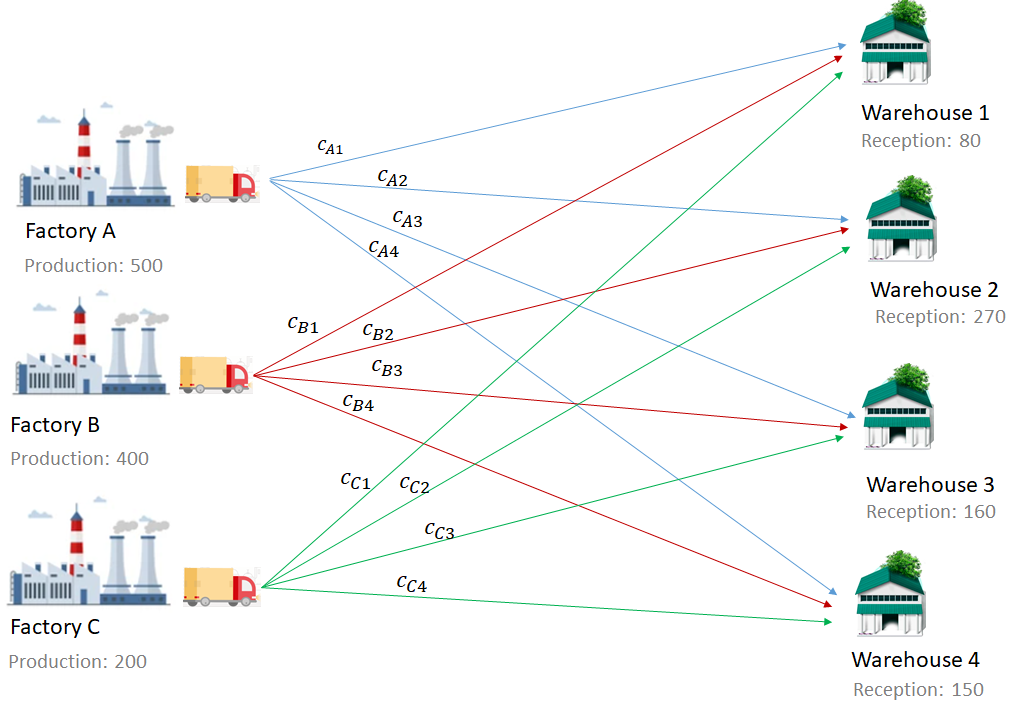
\includegraphics[width=0.85\linewidth]{figures/transport-problem.png}
    \caption{Minh họa về bài toán vận chuyển.}
    \label{fig:flow_network}
\end{figure}

Trước hết, gọi các định lượng $a_1, a_2, ..., a_m$ của một sản phẩm cụ thể cần được gửi đi từ mỗi một $m$ vị trí và nhận với số lượng $b_1, b_2, ..., b_n$ tương ứng tại mỗi $n$ điểm đích. Với mỗi việc giao sản phẩm, một đơn vị sản phẩm từ vị trí nguồn $i$ đến vị trí đích $j$ tiêu hao chi phí $c_{ij}$. Gọi $x_{ij}$ là số sản phẩm giao giữa mỗi cặp vị trí nguồn và đích, $i= 1...m$ và $j=1...n$; cần phải tìm $x_{ij}$ để thỏa mãn yêu cầu vận chuyển và cực tiểu tổng chi phí của công việc vận chuyển. Và ta có bài toán quy hoạch tuyến tính như sau:

\begin{equation}
    \label{eq:transport_problem}
    \begin{aligned}
        \text{minimize } \quad & \sum_{ij} c_{ij}x_{ij}\\
        \text{subject to }\quad & \sum_{j=1}^nx_{ij} = a_i, i = 1, ...m \\ 
        & \sum_{i=1}^mx_{ij} = b_j, j = 1, ...n \\ 
            & x_{ij} \geq 0, i = 1, ...m; j = 1, ...n
    \end{aligned}   
\end{equation}

\subsection{Bài toán luồng cực đại - Maximal Flow Problem}

Có một số bài toán thực tế có thể được mô hình hóa dưới dạng các luồng trong đồ thị đặc biệt gọi là luồng trên mạng. Luồng trên mạng là một đồ thị có hướng có các cạnh được dán nhãn bằng các số không âm biểu thị thông lượng của một loại dòng chảy nào đó: năng lượng điện, hàng hóa sản xuất sẽ được phân phối hoặc phân phối nước thành phố. Hình \ref{fig:flow_network} là một ví dụ trừu tượng về luồng trên mạng.

\begin{figure}[h!]
    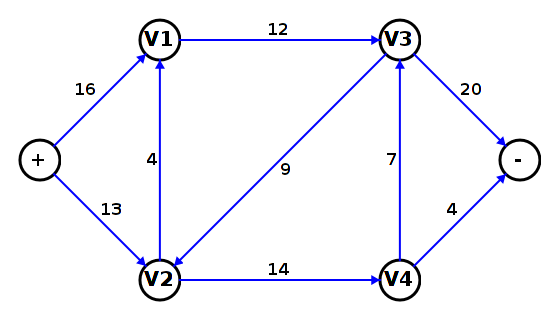
\includegraphics[width=0.85\linewidth]{figures/flow-network.png}
    \caption{Minh họa về một luồng trên mạng.}
    \label{fig:flow_network}
\end{figure}

Mạng luồng có thể có các đỉnh đặc biệt gọi là nguồn (sources) và đích (sinks).
\begin{itemize}
    \item Một nguồn tạo ra hoặc tạo ra bất cứ thứ gì đang chảy trong mạng. Đỉnh "+" thể hiện điểm nguồn trong luồng trên mạng trong Hình \ref{fig:flow_network}. Tùy thuộc vào bản chất chính xác của vấn đề, nguồn cũng có thể có giới hạn hoặc công suất.
    \item Một đích tiêu thụ bất cứ thứ gì đang chảy trong mạng. Đỉnh "-" thể hiện điểm đích trong luồng trên mạng trong Hình \ref{fig:flow_network}. Tùy thuộc vào bản chất chính xác của vấn đề, điểm đích cũng có thể có giới hạn hoặc dung tích.
\end{itemize}

Nút nguồn và nút đích của một mạng là phân biệt nhau, ta gọi chúng lần lượt là nút 1 và nút $m$. Tất cả các nút còn lại phải thỏa mãn điều kiện rằng lưu lượng vào chúng bằng 0. Tuy nhiên, nút nguồn có một luồng lưu lượng ra và nút đích có một luồng lưu lượng vào. Luồng lưu lượng ra $f$ của nút nguồn sẽ bằng luồng lưu lượng vào của nút đích như một hệ quả vì điều kiện của các nút còn lại. 

Một tập hợp các luồng cung thỏa mãn các điều kiện này được gọi là một luồng trong mạng có giá trị $f$. Bài toán luồng cực đại là vấn đề xác định luồng cực đại có thể được thiết lập trong mạng như vậy.

\begin{equation}
    \label{eq:transport_problem}
    \begin{aligned}
        \text{maximize } \quad & f\\
        \text{subject to }\quad & \sum_{j=1}^nx_{1j} - \sum_{j=1}^nx_{j1} - f = 0\\ 
        & \sum_{j=1}^nx_{ij} - \sum_{j=1}^nx_{ji} = 0, i \ne 1, m \\
        & \sum_{j=1}^nx_{mj} - \sum_{j=1}^nx_{jm} + f = 0 \\
            & 0 \leq x_{ij} \leq k_{ij}, \forall i, j
    \end{aligned}   
\end{equation}

\subsection{Bài toán chuỗi cung ứng - Supply-Chain Problem}

\subsection{Bài toán tối ưu phân lớp tuyến tính và Support Vector Machine}

\begin{figure}[h!]
    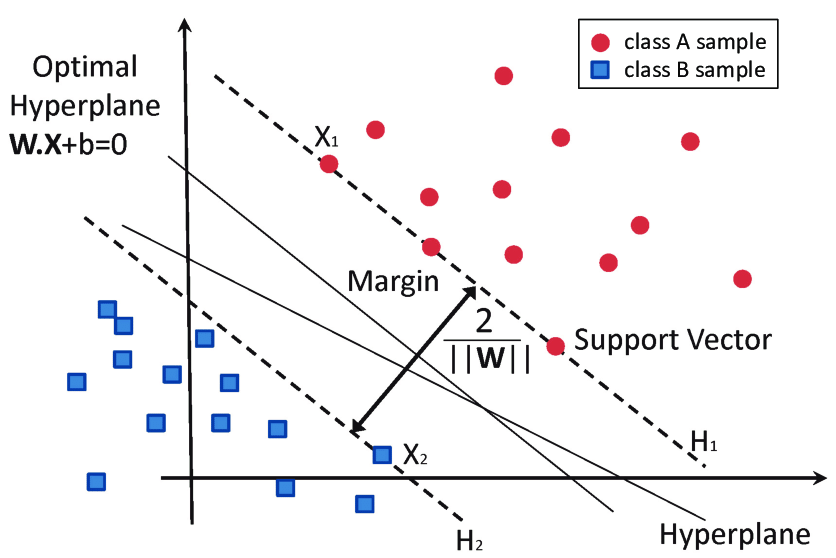
\includegraphics[width=0.85\linewidth]{figures/svm.png}
    \caption{Minh họa về support vector machine.}
    \label{fig:flow_network}
\end{figure}

    % Chương 4
    \chapter{PHƯƠNG PHÁP LẬP TRÌNH}


    % Chương 5
    \chapter{PHƯƠNG PHÁP ĐƠN HÌNH}

Trong chương này, chúng tôi trình bày ý tưởng của thuật toán đơn hình và áp dụng giải quyết bài toán quy hoạch tuyến tính trong không gian hai chiều.

\section{Ý tưởng thuật toán}


\section{Ví dụ minh họa thuật toán}


\section{Bàn luận về thuật toán}

    % Chương 6
    \chapter{PHƯƠNG PHÁP LẬP TRÌNH CHO QUY HOẠCH TUYẾN TÍNH}

Trong chương này, chúng tôi trình bày ví dụ minh họa trong việc sử dụng ngôn ngữ lập trình Python và thư viện bộ giải Gurobi\cite{gurobi}.

\section{Cài đặt phần mềm}

Trước tiên, chúng ta cần có sẵn môi trường Python. Sau đó, chúng ta sẽ cài đặt thư viện Gurobi. Gurobi là một trong những công cụ giải quyết tối ưu hóa mạnh mẽ và nhanh nhất và công ty liên tục tung ra các tính năng mới. Câu lệnh cài đặt như sau
\begin{mintedbox}{python}
python -m pip install -i https://pypi.gurobi.com gurobipy==10.0
\end{mintedbox}

\section{Bài toán quy hoạch tuyến tính}

Xem xét một công ty sản xuất sản xuất hai mặt hàng: cốc và đĩa. 
\begin{itemize}
    \item Sau khi làm xong, một chiếc cốc được bán với giá 27 USD và một chiếc đĩa được bán với giá 21 USD.
    \item Để làm ra mỗi chiếc cốc, chi phí vật liệu là 10 USD và nhân công là 14 USD.
    \item Để làm ra mỗi chiếc đĩa, chi phí vật liệu là 9 USD và nhân công là 10 USD.
    \item Để làm ra mỗi chiếc cốc, phải mất 2,2 giờ lao động.
    \item Để làm ra mỗi chiếc đĩa, phải mất 1 giờ lao động.
    \item Hãng có nguồn cung nguyên liệu vô hạn.
    \item Do số lượng công nhân có hạn nên một công ty có tối đa 100 giờ lao động.
    \item Nhu cầu về cốc là không giới hạn nhưng nhu cầu về đĩa là 30 chiếc.
\end{itemize}

Mục tiêu của công ty là tối đa hóa lợi nhuận (doanh thu – chi phí).

\section{Giải bài toán}

\subsection{Bước 1 - Định nghĩa các biến}

\begin{mintedbox}{python}
# Create variables
x1 = m.addVar(name="x1")
x2 = m.addVar(name="x2")
\end{mintedbox}

\subsection{Bước 2 - Định nghĩa hàm mục tiêu}

\begin{mintedbox}{python}
# Set objective
m.setObjective(3*x1 + 2*x2 , GRB.MAXIMIZE)
\end{mintedbox}

\subsection{Bước 3 - Định nghĩa các ràng buộc bất đẳng thức}

\begin{mintedbox}{python}
# Build (sparse) constraint matrix
m.addConstr(2.2*x1 + x2  <= 100, "c1")
m.addConstr(x2  <= 30, "c3")
m.addConstr(x1  >= 0, "c4")
m.addConstr(x2  >= 0, "c5")
\end{mintedbox}

\section{Chương trình hoàn thiện và thực nghiệm}

Toàn bộ mã nguồn và kết quả thực nghiệm

\begin{figure}[h!]
    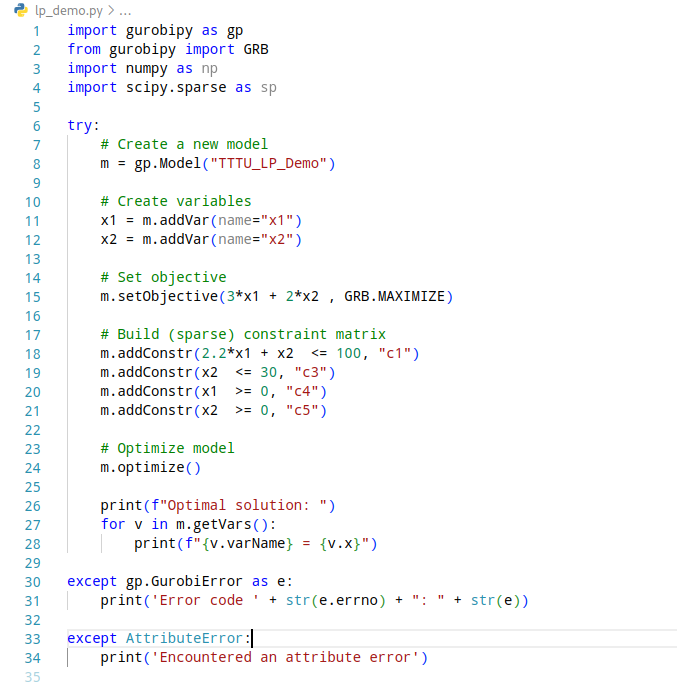
\includegraphics[width=0.85\linewidth]{figures/lp_demo1.png}
    \caption{Mã nguồn chương trình.}
    \label{fig:lp_demo1}
\end{figure}

\begin{figure}[h!]
    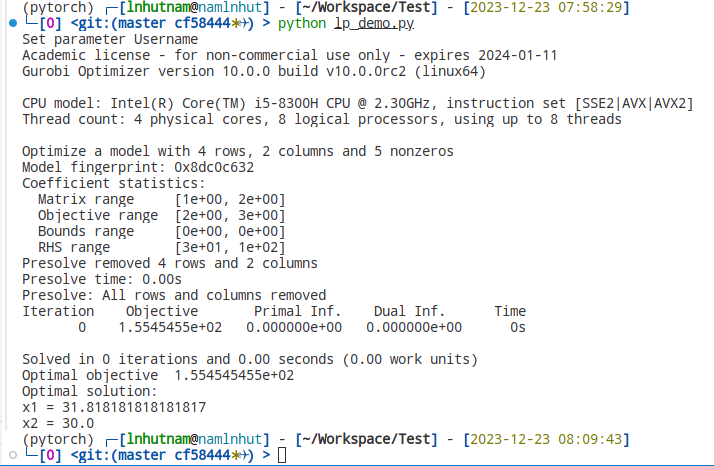
\includegraphics[width=0.85\linewidth]{figures/lp_demo2.png}
    \caption{Kết quả thực nghiệm.}
    \label{fig:lp_demo2}
\end{figure}

    % Chương 7
    \chapter{MỘT SỐ ỨNG DỤNG CỦA QUY HOẠCH TUYẾN TÍNH}

    % Chuong 8
    \chapter{KẾT LUẬN VÀ HƯỚNG NGHIÊN CỨU TƯƠNG LAI}

    % Danh mục công bố công trình
    % \chapter*{DANH MỤC CÔNG TRÌNH CỦA TÁC GIẢ}
\addcontentsline{toc}{chapter}{{\bf DANH MỤC CÔNG TRÌNH CỦA TÁC GIẢ}}

    % Tài liệu tham khảo
    \refs
    \nocite{*}

    % Phụ lục
    % \appendix

\chapter*{PHỤ LỤC 1: NỘI SUY HERMITE}
\addcontentsline{toc}{chapter}{{\bf PHỤ LỤC 1: NỘI SUY HERMITE}}

Giả định rằng tại một điểm cho trước $x_j$, ta biết một giá trị hàm $y_i$, và có thể có nhiều giá trị đạo hàm $y_j', y''_j, \dots, y_j^{m_j}$. Ta có thể sử dụng ma trận Vandermonde để chứng tỏ rằng tồn tại một đa thức duy nhất $P$ với bậc không nhỏ hơn $d$ mà thỏa mãn
\begin{equation}
    P^{(k)}(x_j) = y^{(k)}_j, k = 0, 1, \dots, m_j, j = 0, 1, \dots, n
\end{equation}
trong đó $d = n + m_0 + m_1 + \dots + m_m$. Đa thức osculating (kissing) là một đa thức nội suy rất tổng quát.

Thật vậy, ta có thể đặt tên cho loại đa thức xấp xỉ được gắn với mỗi loại dữ liệu và cho bậc của chúng.
\begin{enumerate}
    \item $n >0$, $m_j = 0$, $j = 0, 1, \dots, n$
    \item $n >0$, $m_j = 1$, $j = 0, 1, \dots, n$
    \item $n = 0$, $n_0 = N$
\end{enumerate}

Khối Vandermonde liên kết với thành phần $j$ bây giờ có $1 + m_j$ dòng, và
\begin{equation}
    \begin{bmatrix}
         1&  x&  x^2&  x^3& \dots & x^d\\ 
         0&  1&  2x&  3x^2& \dots&dx^{d-1}\\ 
         0&  0&  2&  6x&\dots &d(d-1)x^{d-2}\\ 
         &  &  &   & \vdots&
    \end{bmatrix}
\end{equation}
được đánh giá tại $x = x_j$. Ma trận Vandermonde $(d+1) \times (d+1)$ này là không suy biến nếu và chỉ nếu $x_j$ phân biệt.

Trong một số ứng dụng, $y_i$ là những giá trị của một hàm đã biết $f$. Nếu $f \in C^{d + 1}([a, b])$, và $[a, b]$ chứa tất cả các điểm, thì $\forall x \in [a, b], \exists\xi \in [a,b]$ sao cho
\begin{equation}
    f(x) = P(x) + \frac{f^{(d+1)}(\xi)}{(d+1)!}\prod_{j=0}^n(x-x_j)^{m_j+1}
\end{equation}

Việc sử dụng một đa thức để nội suy một tập hợp lớn các điểm (hoặc một số lượng lớn các điều kiện trên một tập hợp điểm) đòi hỏi bộ nội suy phải có bậc lớn. Điều này thường tạo ra các dao động lớn và không mong muốn trong bộ nội suy và khiến việc đánh giá $P(x)$ tốn kém hơn. Nếu ta có quyền tự do lựa chọn các nút, chúng có thể được chọn để giảm thiểu các dao động dữ dội; đây được gọi là lựa chọn nút Chebyshev.

\chapter*{PHỤ LỤC 2: THIẾT LẬP CÁC CHẶN SAI SỐ CHO NỘI SUY HERMITE}
\addcontentsline{toc}{chapter}{{\bf PHỤ LỤC 2: THIẾT LẬP CÁC CHẶN SAI SỐ CHO NỘI SUY HERMITE}}


\section{Chứng minh 2}


\chapter*{PHỤ LỤC 3: LÝ THUYẾT CƠ BẢN VỀ XẤP XỈ ĐA THỨC}
\addcontentsline{toc}{chapter}{{\bf PHỤ LỤC 3: LÝ THUYẾT CƠ BẢN VỀ XẤP XỈ ĐA THỨC}}

Xem xét một không gian tuyến tính (linear space) không nhất thiết phải là không gian hữu hạn chiều (finte dimensional space) mà các phần tử của nó là các hàm $\{f(x)\}$. Chuẩn (norm) được định nghĩa là một phép gán một số thực vào mỗi phần tử của không gian tuyến tính trên, ký hiệu $\text{Norm}(f) \equiv N(f) \equiv \left \|  f\right \|$ thỏa mãn:
\begin{itemize}
    \item $\left \|  f\right \| \geq 0$,
    \item $\left \|  f\right \| = 0$ nếu và chỉ nếu $f(x) \equiv 0$,
    \item $\left \|  cf\right \| =  \left | c \right |\cdot \left \|  f\right \|$, với mọi hằng số $c \in \R$,
    \item $\left \|  f + g\right \| \leq \left \|  f\right \| + \left \|  g\right \|$
\end{itemize}

Một độ đo của độ lệch chuẩn (measure of the deviation) hay độ lỗi (error) trong một xấp xỉ của $f(x)$ bởi $P_n(x)$ được định nghĩa một cách tổng quát bởi khái niệm bán chuẩn (semi-norm):
\begin{equation}
    \left | f(x) - P_n(x) \right |_{sn}
\end{equation}

Ta giả định rằng các đa thức và hàm, $f(x)$, cần được xấp xỉ trong một không gian tuyến $C[a, b]$ của các hàm đươc định nghĩa trên một khoảng bị chặn đóng, $[a, b]$. 

\begin{theorem}
    \label{theorem:3.0.0}
    Gọi một độ đo của độ lệch chuẩn $\left | . \right |_{sn}$ được định nghĩa trong $C[a, b]$, và tồn tại các số dương $m_n$ và $M_n$ thỏa mãn:
    \begin{equation}
        0 < m_n \leq \left | \sum_{j=0}^nb_jx^j \right |_{sn} \leq M_n, n = 0, 1, \dots
    \end{equation}
    với mọi $\{b_j\}$ mà thỏa mãn
    \begin{equation}
        \sum_{j=0}^nb_j = 1
    \end{equation}
    Thì với bất kỳ số nguyên $n$ và $f(x)$ trong $C[a, b]$, tòn tại một đa thức bậc lớn nhất $n$ mà
    \begin{equation}
        d_n = \left | f(x) - P_n(x) \right |_{sn}
    \end{equation}
    đạt được giá trị nhỏ nhất trên tất cả các đa thức.
\end{theorem}

Một nhận xét: hàm $f(x)$ không nhất thiết phải liên tục. Hơn nữa, định lý trên không cho một ước lượng về độ lớn của $d_n$. 

Về các kết quả về tính duy nhất, ta cần độ đo của độ lệch chuẩn nên nghiêm ngặt (strict). Bằng cách định nghĩa một chuẩn $\left | .\right |_{sn}$ là nghiêm ngặt nếu
\begin{equation}
    \left | f+g\right |_{sn} = \left | f\right |_{sn} + \left | g\right |_{sn}
\end{equation}
dẫn đến tồn tại các hằng $\alpha, \beta$ mà $\left | \alpha\right | + \left | \beta\right | \ne 0$ và 
\begin{equation}
    \alpha f(x) + \beta g(x) \equiv 0
\end{equation}

Ta có định lý sau. 
\begin{theorem}
    Giả thiết của định lý \ref{theorem:3.0.0} thêm vào yêu cầu $\left | .\right |_{sn}$ là nghiêm ngặt. Thì đa thức nhỏ nhất, gọi là $P_n(x)$ là duy nhất.
\end{theorem}

\section{Định lý xấp xỉ Weierstrass và Đa thức Bernstein}

Định lý xấp xỉ Weierstrass được phát biểu như sau:
\begin{theorem}
    \label{theorem:weierstrass_approx}
    Gọi $f(x)$ là bất kỳ hàm liên tục nào trong khoảng (đóng) $[a, b]$. Thì với bất kỳ $\epsilon > 0$, tồn tại một số nguyên $n = n(\epsilon)$ và một đa thức $P_n(x)$ với bậc cao nhất $n$ thỏa
    \begin{equation}
        \left | f(x) - P_n(x)\right | < \epsilon
    \end{equation}
    với mọi $x \in [a, b]$
\end{theorem}

Định lý \ref{theorem:weierstrass_approx} đảm bảo có thể xấp xỉ đa thức gần thông qua một khoảng giới hạn đóng chỉ với điều kiện là hàm được xấp xỉ là liên tục. Phát biểu của định lý là về sự tồn tại và không cho một gợi ý nào về cách xây dựng những xấp xỉ. Tuy nhiên, một chứng minh đơn giản và tao nhã của kết quả này do Bernstein trình bày trong định lý

Đa thức Bernstein bậc $n$ cho hàm $f(x)$ trên $[0, 1]$ được định nghĩa:
\begin{equation}
    B_n(f; x) \equiv \sum_{j = 0}^nf(x_j)\beta_{n, j}(x)
\end{equation}
với 
\begin{equation}
    \beta_{n, j}(x) = \binom{n}{j}x^j(1-x)^{n-j}
\end{equation}
\begin{theorem}
    Gọi $f(x)$ là bất kỳ hàm liên tục nào được định nghĩa trên $[0, 1]$. Thì với mọi $x \in [0, 1]$, và bất kỳ số nguyên dương $n$ nào,
    \begin{equation}
        \left | f(x) - B_n(f; x)\right | \leq \frac{9}{4}\omega(f;n^{-1/2})
    \end{equation}
    trong đó modulus của tính liên tục của $f(x)$ trong $[0, 1]$ được định nghĩa
    \begin{equation}
        \omega(f; \delta) = \underset{x, x' \in [0, 1], \left | x - x'\right | \leq \delta}{\text{Least-upper-bound}}\left | f(x) - f'(x)\right |
    \end{equation}
\end{theorem}
Định lý xấp xỉ Weierstrass được suy ra nhờ chọn $n$ đủ lớn sao cho $\omega(f;n^{-1/2}) < \frac{4\epsilon}{9}$.

Nếu $f(x)$ thỏa mãn điều kiện Lipschitz, ta dễ dàng tìm được
\begin{coro}
    Gọi $f(x)$ thỏa mãn điều kiện Lipschitz
    \begin{equation}
        \left | f(x) - f(y)\right | \leq \lambda\left | x-y\right |
    \end{equation}
    với mọi $x, y \in [0, 1]$. Thì với mọi $x\in [0, 1]$
    \begin{equation}
        \left | f(x) - B_n(f; x)\right | \leq  \frac{9}{4}\lambda n^{-1/2}.
    \end{equation}
\end{coro}

\section{Xấp xỉ bình phương tối tiểu}

\begin{theorem}
    Với mỗi hàm chính xác $f(x)$, tồn tại một xấp xỉ đa thức bình phương tối tiểu duy nhất bậc tối đa $n$ mà cực tiểu
    \begin{equation}
        \left \| f(x) - Q_n(x) \right \|_2 \equiv \left\{\int_a^b[f(x) - Q_n(x)]^2dx\right\}^{\frac{1}{2}}
    \end{equation}
\end{theorem}

\begin{theorem}
    Hệ số của ma trận $H_{n+1}(a,b)$ là không suy biến.
\end{theorem}

\begin{theorem}
    Gọi $f(x)$ là liên tục trên $[a, b]$ và $Q_n(x), n=0,1,\dots,$ là đa thức xấp xỉ bình phương tối tiểu đến $f(x)$ trên $[a,b]$. Thì
    \begin{equation}
        \lim_{n \rightarrow \infty}J_n \equiv \lim_{n \rightarrow \infty}\int_a^b[f(x) - Q_n(x)]^2dx = 0
    \end{equation}
    và ta có phương trình Parseval
    \begin{equation}
        \int_a^bf^2(x)dx = \sum_{j =0}^{\infty}c_j^2
    \end{equation}
\end{theorem}

\section{Các đa thức của xấp xỉ "tốt nhất"}

Một độ đo của độ lệch chuẩn giữa một hàm $f(x)$ và một đa thức xấp xỉ bậc $n$, $P_n(x) = a_0 + a_1x + \dots + a_nx^n$ là chuẩn cực đại (maximum norm):
\begin{equation}
    \label{eq:max_norm}
    \left \| f(x) - P_n(x) \right \|_{\infty}  \equiv \underset{a\leq x\leq b}{\max}\left | f(x) - P_n(x) \right | \equiv D(f, P_n)
\end{equation}
Khi một đa thức nào đó mà cực tiểu chuẩn này thì được gọi là đa thức của xấp xỉ "tốt nhất".

Phương trình \eqref{eq:max_norm} định nghĩa các hệ số $\{a_i\}$ không tường minh
\begin{equation}
    d(a_0, a_1, \dots, a_n) \equiv \underset{a\leq x\leq b}{\max}\left | f(x) - P_n(x) \right |
\end{equation}

Một đa thức xấp xỉ tốt nhất được đặc trưng bởi một điểm $\Bar{\mathbf{a}}$ trong không gian $(n+1)$ mà $d(\mathbf{a})$ nhỏ nhất. Định lý sau khẳng định sử tồn tại của đa thức như thế.
\begin{theorem}
    Gọi $f(x)$ là một hàm liên tục trong khoảng $[a,b]$. Thì với bất kỳ số nguyên $n$ nào, tồn tại một đa thức $\hat{P}_n(x)$, bậc tối đa $n$, mà cực tiểu được chuẩn:
    \begin{equation}
        \left \| f(x) - P_n(x) \right \|_{\infty}
    \end{equation}
\end{theorem}

\section{Xấp xỉ lượng giác}

Ta nói $S_n(x)$ là một tổng lượng giác bậc tối đa $n$, nếu
\begin{equation}
    \label{eq:trigonometric_sum}
    S_n(x) = \frac{1}{2}a_0 + \sum_{k=1}^n(a_k\cos(kx) + b_k\sin(kx))
\end{equation}
Bằng cách sử dụng hàm mũ
\begin{align}
    \begin{aligned}
        e^{i\theta} &\equiv \cos\theta + i\sin\theta\\
        \cos\theta &= \frac{1}{2}(e^{i\theta} + e^{-i\theta})\\
        \sin\theta &= \frac{-i}{2}(e^{i\theta} - e^{-i\theta})\\
    \end{aligned}
\end{align}
thì phương trình \eqref{eq:trigonometric_sum} có thể được viết một cách đơn giản hơn
\begin{equation}
    S_n(x) = \sum_{k=-n}^nc_ke^{ikx}
\end{equation}
với 
\begin{align}
    \begin{aligned}
        c_0 &= \frac{a_0}{2}\\
        c_k &= \frac{1}{2}(a_k - ib_k)\\
        c_{-k} &=  \frac{1}{2}(a_k + ib_k)\\
        & k = 1, 2, \dots, n
    \end{aligned}
\end{align}
Kết quả cơ bản trong xấp xỉ bởi tổng lượng giác dựa trên Weierstrass, và có thể được phát biểu thông qua định lý dưới đây:
\begin{theorem}
    Gọi $f(\theta)$ liên tục trên khoảng $[-\pi, \pi]$, và tuân theo chu kỳ $2\pi$. thì với bất kỳ $\epsilon > 0$, tồn tại một $n = n(\epsilon)$ và một tổng lượng giác, $S_n(\theta)$ sao cho
    \begin{equation}
        \left | f(\theta) - S_n(\theta) \right | < \epsilon
    \end{equation}
    với mọi $\theta$.
\end{theorem}

\subsection{Nội suy lượng giác}

\subsection{Xấp xỉ lượng giác bình phương tối tiểu. Chuỗi Fourier}

\subsection{Xấp xỉ lượng giác "tốt nhất"}

Nếu hàm $f(x)$ liên tục trên $[-\pi, \pi]$, ta có thể tìm một tổng lượng giác bậc $n$ mà cực tiểu chuẩn cực đại
\begin{equation}
    \left \| f(x) - S_n(x) \right \|_{\infty}  = \underset{-\pi\leq x\leq \pi}{\max}\left | f(x) - S-n(x) \right |
\end{equation}
Sự tồn tại của đa thức này có thể được xác minh bằng cách sử dụng 



\end{document}